%!TEX root = ../template.tex
%%%%%%%%%%%%%%%%%%%%%%%%%%%%%%%%%%%%%%%%%%%%%%%%%%%%%%%%%%%%%%%%%%%%
%% chapter3.tex
%% NOVA thesis document file
%%
%% Chapter with a short latex tutorial and examples
%%%%%%%%%%%%%%%%%%%%%%%%%%%%%%%%%%%%%%%%%%%%%%%%%%%%%%%%%%%%%%%%%%%%

\typeout{NT FILE chapter3.tex}%

\makeatletter
\newcommand{\ntifpkgloaded}{%
  \@ifpackageloaded%
}
\makeatother

\chapter{Trabalho Relacionado}
\label{cha:trabalho_relacionado}

No vigésimo-quinto USENIX Security Symposium, foi apresentada por Philipp Winter et al, em 2016, uma análise da rede Tor nos anos anteriores, que permitiu a deteção de nós \textit{Sybil} e a sua categorização graças à ferramenta denominada de \textit{sybilhunter} \cite{winter2016identifying}. Um dos grupos de nós \textit{Sybil} foram denominados de \textbf{“FDCservers”}, que tinham como objetivo individualizar e identificar utilizadores de \textit{onion services}, validando a hipótese que é um ataque recente e que continua até aos dias de hoje a ser uma ameaça à rede Tor.

Em 2002, Douceur argumenta que é praticamente impossível haver defesa contra \textit{Sybil attacks} sem uma autoridade central e confiável que ateste uma ligação de um para um entre identidade e entidade \cite{douceur2002sybil}. Com o uso de ZKPs, \textit{verifiable credentials} e inteligência artificial, surgem novas soluções que podem contestar essa afirmação.

Para averiguar melhor a solução proposta, é necessário avaliar soluções passadas para mitigar e prevenir \textit{Sybil attacks}, de forma a consciencializar o leitor relativamente ao estado da arte até ao momento.

\section{Técnicas de Prevenção de Sybil Attacks até hoje}
\label{sec:tecnicas_prevencao_sybils}

Nas próximas categorias estão presentes várias técnicas de deteção, prevenção e mitigação de \textit{Sybil attacks} até atualmente, que foram exploradas por diferentes investigadores da área da computação, englobando técnicas de autenticação centralizadas, mecanismos de deteção de possíveis nós \textit{Sybil} na rede Tor até uso de inteligência artificial \cite{levine2006survey}.

\subsection{Certificação Confiável}
\label{ssec:certificacao_confiavel}

Como provado por Douceur, até à data era impossível prevenir \textit{Sybil attacks} sem uma entidade autoritária confiável que emitisse certificados que validassem a identidade de \textit{relay operators}, garantindo que cada uma estaria apenas conectada a uma entidade na rede \cite{douceur2002sybil}. Douceur não apresenta nenhuma solução que permita garantir esta unicidade de entidade, senão o uso de processos manuais ou em pessoa para tal, surgindo eventuais limitações de segurança e performance. Neste âmbito, surgem soluções como:

\begin{itemize}
  \item \textit{\textbf{Farsite:}} Desenvolvido por Atul Adya et al no mesmo ano da publicação de Douceur, o \textit{Farsite} \cite{adya2002farsite} surge como um sistema de ficheiros escalável centralizado, embora fisicamente distribuído entre um conjunto de computadores que não se podem presumir confiáveis. A autoridade central e confiável faz uso de vários tipos de certificados de criptografia assimétrica emitidos pela mesma, associando-os a peças de identificação de ficheiros e da máquina, eliminando possíveis \textit{sybils} dos mesmos;
  \item \textit{\textbf{Secure routing for structured peer-to-peer overlay networks:}} Desenvolvido por Miguel Castro et al também no mesmo ano da publicação de Douceur, este \textit{paper} estuda ataques direcionados à prevenção da entrega de mensagens de forma correta em \textit{peer-to-peer overlays} estruturados, mencionando possíveis defesas \cite{castro2002secure}. De forma a defender a rede relativamente a \textit{Sybil attacks}, são usados um conjunto de \textit{certification authorities} (CA) como entidade autoritária central para emissão de certificados de identificação de nós, conectando-os a uma chave pública. Para além disso, mencionam o uso de tarifas monetárias para a emissão de certificados (este tipo de mitigação de ataques será discutido em mais detalhe no tópico das \textit{Nym Credentials}), de forma a tornar este tipo de ataque insustentável para o atacante, financiando também as CA. Como segunda opção, refere-se a ligação entre os identificadores dos nós com a identificação no mundo real;
  \item \textit{\textbf{XenoTrust}} Desenvolvido por Boris Dragovic et al, o \textit{XenoTrust} surge como uma arquitetura confiável de \textit{management} usada na \textit{XenoServer Open Platform} , isto é uma infraestrutura pública para computação em grande área, de forma a lidar com \textit{tasks} compreendidas no espetro inteiro de paradigmas distribuídos \cite{dragovic2003xenotrust}. Depois do projeto ter sido apresentado, é discutida a sua tolerância a \textit{Sybil attacks} \cite{dragovic2003managing}, sendo apresentados dois motivos:
  \subitem É usada uma agência autoritária central confiável, denominada de \textit{XenoCorp}, que valida todas as identidades usadas na plataforma. Para registar múltiplas identidades, era necessário apresentar o mesmo número de identidades legais independentes entre si;
  \subitem Como é usado um sistema baseado em reputação, é difícil para o atacante determinar o impacto do ataque de forma precisa, resultando em dificuldade em controlar os custos de múltiplas identidades.
  \item \textit{\textbf{Securing Routing in Open Networks Using Secure Traceroute:}} Proposto por Gaurav Mathur et al em 2004, esta aplicação de um \textit{secure traceroute protocol} para detetar e localizar \textit{faulty packet forwarding} discute uma análise de segurança em que é assumida uma técnica de autenticação entre nós honestos graças a \textit{verifiable credentials} conectadas às identidades dos nós, que não podem ser reemitidas caso perdidas \cite{mathur2004securing};
  \item \textit{\textbf{A Framework for Dynamic Byzantine Storage:}} Apresentado por Jean-Philippe Martin et al, é proposto uma arquitetura de transformação de vários protocolos baseados em quóruns que adapta automaticamente o seu limite de falhas e contador de servidor, de forma a reconfigurar previamente a falhas ou para substituir outros servidores \cite{martin2004framework}. Esta arquitetura previne \textit{Sybil attacks} ao identificar previamente os servidores antes de se juntarem ao sistema;
  \item \textit{\textbf{On the Utility of Distributed Cryptography in P2P and MANETs:}} Este projeto explora as dificuldades em autenticação de membros de uma rede em redes descentralizadas, com outros problemas relativos à segurança, utilizando \textit{threshold cryptography} para controlo de membros em sistemas \textit{peer-to-peer} \cite{narasimha2003utility}. O problema de identidades \textit{sybil} surge na impersonificação de várias identidades por só um membro da rede, que sugerem ser mitigado a partir de certificação dentro do contexto do projeto para que o utilizador se possa conectar à mesma;
  \item \textit{\textbf{Incentives and fair sharing in peer-to-peer systems:}} Este projeto explora uma arquitetura de sistemas \textit{peer-to-peer} que visa a partilha de recursos computacionais dentro da rede \cite{ngan2004incentives}. Para mitigar possíveis \textit{Sybil attacks}, faz uso de uma autoridade central confiável, CA, para emissão de permissões de entrada;
  \item \textit{\textbf{Transaction-based Charging in Mnemosyne:}} Timothy Roscoe e Steven Hand apresentam o \textit{Mnemosyne}, um sistema estenográfico de armazenamento \textit{peer-to-peer}, de forma a que os ficheiros de um utilizador não possam existir sem uma chave. Os nós do \textit{Mnemosyne} são assumidos como servidores controlados ou por um service provider ou por um grupo de providers com reputação conhecida, conotando os clientes como utilizadores do sistema que não participam na rede \textit{peer-to-peer}. Esta divisão permite que os servidores possam ser identificados a partir de certificados, evitando \textit{Sybil attacks} \cite{roscoe2002transaction};
  \item \textit{\textbf{Admission control in Peer-to-Peer:}} Explorado por Nitesh Saxena et al, este \textit{paper} visa construir e avaliar mecanismos de admissão de \textit{peer-to-peer} baseados em várias técnicas criptográficas, com uma análise principalmente focada em \textit{performance}, apesar de referenciar também anonimidade, \textit{unlinkability} e \textit{accountability}, concluindo que na data em que foi publicado, 2003, ainda não era possível fazer autenticação de \textit{peers} numa rede \textit{peer-to-peer} de forma criptograficamente avançada \cite{saxena2003admission}. O método de uma autoridade central para emissão de certificados torna-se então fulcral para a evasão de \textit{Sybil attacks};
  \item \textit{\textbf{HOURS:}} Por Hao Yang et al, é apresentado o \textit{HOURS}, uma arquitetura que garante resiliência contra \textit{Denial-of-Service} attacks numa hierarquia aberta de serviço \cite{yang2004hours}, mitigando possíveis ataques de \textit{Sybil} a partir do uso de \textit{random hash functions}, estilo SHA-1, para mapear o nome do nó até ao seu identificador, de modo a que o atacante não tenha permissão para o escolher, restringindo o controlo do mesmo na admissão de controlo;
  \item \textit{\textbf{Tapestry:}} Este projeto é apresentado como uma infraestrutura de \textit{peer-to-peer overlay routing} que oferece eficiência, escalabilidade, e independente da localização diretamente para cópias de recursos localizados \cite{zhao2004tapestry}. Neste caso, fazem uso de uma \textit{public-key infrastructure}, PKI, para mapear as chaves aos identificadores dos nós;
  \item \textit{\textbf{Secure routing in wireless sensor networks:}} É proposto um protocolo de \textit{routing} para uma rede de sensor com objetivo na segurança, propondo também objetivos de segurança para \textit{routing} neste tipo de redes. A mitigação de \textit{Sybil attacks} é feita a partir da adição de uma camada de encriptação e autenticação usando uma chave partilhada globalmente \cite{karlof2003secure}.
\end{itemize}

Estes são alguns dos projetos que fazem uso deste tipo de solução para os \textit{Sybil attacks}, entre muitos outros que não foram incluídos por serem muito similares aos já apresentados ou porque os autores não fizeram grande ênfase à proteção contra este tipo de ataques. Esta categoria é de longe a mais explorada visto que é a que engloba a maior janela temporal em que não houve muitos avanços nas estratégias de mitigação de \textit{Sybil attacks}, logo muitos projetos fazem uso deste tipo de mecanismo.

\subsection{Sem Solução}
\label{ssec:sem_solucao}

Enquanto grande parte dos projetos apresentados fazem uso da solução genérica apresentada por Douceur, existe uma grande parte que não apresenta nenhuma solução como defesa para eventuais \textit{Sybil attacks} ao sistema:

\begin{itemize}
  \item \textit{\textbf{On the Economics of Anonymity:}} Alessandro Acquisti, Roger Dingledine (co-fundador do Tor Project) e Paul Syverson discutem as razões pelas quais a implementação de sistemas anónimos é difícil, enumeram os incentivos para participar como \textit{senders} ou nós e constroem um modelo geral para descrever os efeitos dos incentivos dados \cite{acquisti2003economics}. Aqui há uma referência ao \textit{Sybil attack} pela nomenclatura de \textit{pseudospoofing}, que era usada anteriormente a esta definição mais concreta, que definem como um “pesadelo” para infraestruturas anónimas que são implementadas a grande escala, não referindo nenhuma solução que possa ser implementada perto da data do \textit{paper} (2003);
  \item \textit{\textbf{Robust Distributed Name Service:}} É apresentado um método chamado \textit{“Trust-but-Verify”} que garante um \textit{distributed name service} robusto, protegido contra ataques em grande escala \cite{awerbuch2004robust}. Contudo, não é apresentada nenhuma solução contra \textit{sybils}, referenciando o método de Douceur embora caracterizando-o como ineficaz;
  \item \textit{\textbf{On the role of contextual information for privacy attacks and classification:}} Este projeto visa definir melhor a ligação entre um utilizador e as suas ações num sistema, de forma a usar a definição como critério de avaliação em grandes conjuntos de dados \cite{cvrcek2004role}. Fazem referência ao \textit{Sybil attack}, mas não apresentam nenhuma solução;
  \item \textit{\textbf{Synchronous Batching:}} Uma vez mais por Roger Dingledine e Paul Syverson, agora com Vitaly Shmatikov, é apresentado um estudo sobre o processo de \textit{batching} prévio à entrada das \textit{MIX networks}, onde argumentam que topologias de \textit{MIXes} de \textit{free-route} garantem mais anonimidade \cite{dingledine2004synchronous}. Neste caso, é apenas referenciado o ataque, nem é explorado como um eventual problema para a solução;
  \item \textit{\textbf{The Architecture of PIER:}} É apresentado um processador de \textit{queries} ao nível da Internet para uso em arquiteturas de \textit{peer-to-peer}, referindo como solução para um \textit{Sybil attack} o uso de identificadores para os clientes de forma centralizada, mas teria resultados pouco eficazes \cite{huebsch2005architecture};
  \item \textit{\textbf{SPROUT:}} O \textit{SPROUT} é um algoritmo de routing por \textit{Distributed Hash Table} para ser usado em redes sociais baseadas em redes \textit{peer-to-peer} \cite{marti2004sprout}. Neste contexto, é enunciado o \textit{Sybil attack} e as suas ameaças para o sistema, mas não é apresentada nenhuma solução;
  \item \textit{\textbf{On dealing with adversaries fairly:}} Este projeto visa explorar os resultados da teoria da escolha social aplicadas a sistemas \textit{peer-to-peer}, e aplica-a a alguns sistemas recomendados na literatura \cite{serjantov2004dealing}, escolhendo categorizar o \textit{Sybil attack} e como o mitigar como \textit{Future Work};
  \item \textit{\textbf{Faithfulness in Internet Algorithms:}} Jeffrey Shneidman et al exploram o conceito de \textit{Faithfulness} quando aplicado a sistemas distribuídos, explorando as diferentes falhas e possíveis manipulações, categorizando o \textit{Sybil attack} como uma delas \cite{shneidman2004faithfulness};
  \item \textit{\textbf{Friends Troubleshooting Network:}} Ao contrário dos anteriores, este projeto visa construir uma \textit{Friends Troubleshooting Network}, que consiste numa rede \textit{peer-to-peer} para que utilizadores possam fazer \textit{troubleshoot} de uma máquina enquanto a privacidade é garantida, enunciado o \textit{Sybil attack} como um ataque possível que, dentro do contexto, pode ser resolvido com a iniciação de vários pedidos para \textit{troubleshoot}, confiando que outros utilizadores reportem os resultados corretos e confiáveis, permitindo que quem faz o pedido consiga fazer distinção entre os emitidos por \textit{sybils} e por clientes fidedignos \cite{wang2004friends}. Este projeto continua nesta categoria porque apresenta uma solução que apenas se adequa ao contexto e confia nos outros utilizadores.
\end{itemize}

É possível concluir que apesar destes projetos já não serem atuais, o \textit{Sybil attack} torna-se um ataque muito comum que afeta o mundo dos sistemas distribuídos e redes de \textit{peer-to-peer} de forma a muitos contextos não encontrarem solução devido à máxima de descentralização da topologia da rede, categorizando a primeira solução como inviável para este tipo de casos.

\subsection{Teste de Recursos}
\label{ssec:teste_recursos}

A ideia desta categoria é identificar possíveis \textit{sybils} com base na tese de que nós independentes têm mais recursos computacionais do que nós controlados pelo mesmo utilizador. Os recursos que são analisados são o poder computacional, o armazenamento, a \textit{network bandwidth} e endereços IP limitados \cite{levine2006survey}. Nesta categoria inserem-se os seguintes casos:

\begin{itemize}
  \item \textit{\textbf{Exposing Computationally-Challenged Byzantine Impostors:}} Este projeto desenvolvido por James Aspnes et al tem como objetivo prevenir \textit{Sybil attacks} em sistemas \textit{peer-to-peer} usando algoritmos distribuídos, mantendo o \textit{Byzantine agreement} a partir de um esquema de \textit{puzzles} moderadamente difíceis como esquema de preços de identificação \cite{aspnes2005exposing}. Estes \textit{puzzles} são uma demonstração de poder computacional, inserindo este caso nesta categoria;
  \item \textit{\textbf{Implementing a Reputation-Aware Gnutella Servent:}} Esta implementação e \textit{design} de um servente à base de reputação para sistemas \textit{peer-to-peer} estilo \textit{Gnutella} faz uso da heterogeneidade de endereços de IP (endereços de IP limitados) para identificação de possíveis nós \textit{sybil} \cite{cornelli2002implementing}.
  \item \textit{\textbf{Tarzan:}} Este projeto consiste numa camada de rede IP \textit{peer-to-peer} que permite anonimizar os clientes de forma descentralizada, \textit{fault-tolerant}, altamente escalável e facilmente gerida, providenciando serviço de IP \cite{freedman2002tarzan}. Para mitigar possíveis \textit{Sybil attacks}, explicam que um adversário não beneficia de correr múltiplos intra-domínios, visto que o \textit{Tarzan} faz mapeamento entre domínios de forma a que não seja possível influenciar as ligações para fora ou para dentro de um nó;
  \item \textit{\textbf{Herbivore:}} Desenvolvido por Sharad Goel et al, este sistema de comunicação \textit{peer-to-peer}, escalável e \textit{tamper-resilient} permite anonimidade e privacidade, baseando-se em redes de \textit{Dining Cryptographers}. Para mitigar \textit{Sybil attacks}, fazem uso de limitações de entradas de nós na rede ao pedirem que completem um desafio computacional \cite{goel2003herbivore};
  \item \textit{\textbf{Preserving Peer Replicas By Rate-Limited Sampled Voting:}} É apresentado um \textit{design} que permite votações em \textit{opinion polls} de forma segura, prevenindo deteção de intrusos previamente a qualquer dano irrecuperável feito ao sistema \cite{maniatis2003preserving}. Os \textit{Sybil attacks} são prevenidos graças a protocolos que requerem que os utilizadores que iniciam as votações e os que votam sejam obrigados a executar operações que aumentem o esforço computacional;
\end{itemize}

Apesar do uso desta técnica, os seus efeitos culminam em desencorajar \textit{Sybil attacks} e não preveni-los. No caso do Tor, esta não é uma solução viável, visto que é possível realizar um ataque com sucesso com apenas duas identidades \cite{wright2004predecessor}.

\subsection{Custos e Taxas Regulares}
\label{ssec:custos_taxas_regulares}

Dentro deste tópico exploramos a revalidação periódica de identidades de nós na rede, de forma a que os nós \textit{Sybil} sejam identificados regularmente:

\begin{itemize}
  \item \textit{\textbf{Group Spreading:}} Apresentado como um protocolo para um serviço distribuído de nomes para ser usado em coleções dinâmicas de \textit{peers} com os seus determinados IDs, este projeto visa deter \textit{Sybil attacks} a partir de uma variação do tópico anterior, usando testes de recursos computacionais periódicos para validação de identidades \cite{awerbuch2004group};
  \item \textit{\textbf{Sufficiently Secure Peer-to-Peer Networks:}} Apresentado por Gatti et al, este projeto determina uma investigação relativa a resistência de censura numa rede \textit{peer-to-peer}, com uma metodologia relativa a \textit{Sybil attacks} que usa mecanismos económicos regulares para validação da identidade \cite{article}.
\end{itemize}

\subsection{Sistemas de Redes Sociais}
\label{ssec:sistemas_redes_sociais}

Apesar de ser uma categoria com menos casos, é relevante mencionar que existem medidas para mitigar \textit{Sybil attacks} com base em sistemas de redes sociais:

\begin{itemize}
  \item \textit{\textbf{SybilGuard:}} Haifeng Yu et al apresentam o \textit{SybilGuard}, um protocolo para limitação de influências corruptoras de \textit{Sybil attacks}, baseando-se numa rede social entre identidades dos utilizadores, onde cada ligação representa uma ligação humana de confiança entre duas identidades \cite{10.1145/1151659.1159945};
  \item \textit{\textbf{Preventing Sybil Attacks by Privilege Attenuation:}} Neste projeto, Philip Fong formaliza o \textit{Denning’s Principle of Privilege Attenuation (POPA)}, que prova ser condição suficiente para prevenir \textit{Sybil attacks} \cite{5958034}. Este princípio, o POPA, tem por base um sistema de rede social no estilo do \textit{Facebook}, que previne o agravamento de privilégios causado por \textit{Sybil attacks} ao exigir que um utilizador apenas possa conceder um privilégio que já tenha obtido.
\end{itemize}

É possível obter uma caracterização mais detalhada de todas as categorias de técnicas de mitigação de \textit{Sybil attacks} \cite{balachandran2012review}, embora as restantes sejam fora do escopo para a solução por apresentar.

\subsection{Recentemente}
\label{ssec:recentemente}

Mais recentemente, surgiram soluções mais avançadas para mitigação de \textit{Sybil attacks}, que apesar de não acrescentar nenhum conhecimento necessário para a solução apresentada, tornam-se interessantes como pontos de partida diferentes para a mesma meta:

\begin{itemize}
  \item \textit{\textbf{Malicious Relay Detection for Tor Network Using Hybrid Multi-Scale CNN-LSTM with Attention:}} Este projeto, desenvolvido em 2023, apresenta um modelo de deteção de \textit{relays maliciosos} denominado de \textit{hybrid multi-scale CNN-LSTM}, com \textit{Attention model (MSC-L-A)}, desenvolvido para a rede Tor \cite{10217886}. Este modelo de aprendizagem faz uso de redes neuronais para inteligência artificial, de forma a facilitar a deteção de \textit{relays} maliciosos, como \textit{sybils}, obtendo os melhores resultados até à data, comparativamente com outros modelos;
  \item \textit{\textbf{Refining Node Similarity Analysis:}} Apresentado em 2024, este projeto visa identificar nós \textit{sybil} a partir das suas similaridades, utilizando um algoritmo que atribui pontuações a nós na rede Tor e usa-as para os comparar entre si, obtendo resultados com alta precisão \cite{sui2024refining};
  \item \textit{\textbf{Impact Analysis of Sybil Attacks in the Tor Network:}} Publicado em 2025, este projeto tem como objetivo analisar o impacto de nós \textit{sybil} na rede Tor a partir de agregação de dados e simulações, caracterizando a situação como um problema de diversidade, visto que grande parte do poder computacional está concentrado entre poucos operadores de \textit{relays} \cite{10.1007/978-3-031-92886-4_13}.
\end{itemize}

Estes estudos mostram que o \textit{Sybil attack} continua a ser um problema recorrente na rede Tor, que ainda é estudado atualmente na tentativa de uso de técnicas emergentes para a sua mitigação.

\section{Coconut}
\label{sec:coconut}

Introduzido em 2018 por Sonnino et al, o \textit{Coconut} surge da necessidade da emissão de credenciais a partir de \textit{smart contracts}, de forma a autenticar a identidade, atributos ou o balanço da conta de um utilizador num modelo \textit{Zero-Knowledge}.

Até à publicação do esquema, outros foram implementados em plataformas que suportam \textit{smart contracts}, como o \textit{Ethereum} \cite{wood2014ethereum}, \textit{Hyperledger} \cite{cachin2016architecture} e \textit{Chainspace} \cite{al2017chainspace}, contudo todos partilham a limitação de que os \textit{verifiable smart contracts} só podem realizar operações em \textit{blockchains} públicas, e que a integridade da segurança do sistema deve-se manter para um número de nós \textit{faulty}, isto é deve ser tolerante a falhas bizantinas, quando esta propriedade deve ser garantida para múltiplos emissores de credenciais \cite{sonnino2018coconut}. Para além disto, as soluções apresentadas não providenciaram eficácia apropriada, \textit{re-randomization}, \textit{blind issuance} (emissão de certificados sem obter conhecimento sobre a entidade que fez o pedido) e capacidade para divulgar informações de forma seletiva. O uso de apenas uma entidade confiável emissora de certificados não previne contra esta se tornar maliciosa, o que se torna uma ameaça para o sistema. Enquanto surgem soluções descentralizadas que previnem esta ameaça, como o esquema de Garman et al \cite{garman2013decentralized}, que permite a emissão de credenciais públicas e verificáveis sem uma entidade central emissora, a limitação de emissão de credenciais e o uso geral das mesmas mantém-se, adicional de métodos de computação extensos para a sua visualização \cite{sonnino2018coconut}.

De forma a enfrentar as adversidades apresentadas \textit{a priori}, o \textit{Coconut} surge como um sistema de divulgação seletiva de credenciais, suportando emissão de credenciais de atributos privados e públicos e \textit{re-randomization}, para auxiliar o uso de várias credenciais sem ligação entre elas.

\begin{figure}[H]
    \centering
    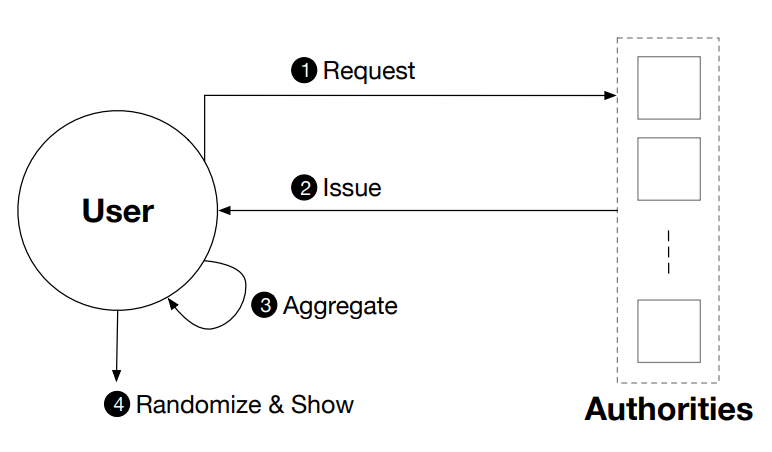
\includegraphics[width=0.7\linewidth]{5-Figures/Coconut.png}
    \caption{Simplificação da arquitetura do Coconut \cite{sonnino2018coconut}.}
    \label{fig:coconut}
\end{figure}

A imagem apresentada permite uma visualização geral simplificada que demonstra o funcionamento do \textit{Coconut}, onde se dividem os seguintes passos \cite{sonnino2018coconut}:

\begin{enumerate}
  \item \textit{\textbf{Request:}} Um utilizador envia um \textit{request} a um conjunto de quaisquer autoridades emissoras de credenciais do \textit{Coconut}, com atributos públicos ou privados, com estes segundos numa modalidade encriptada, para serem atribuídos à credencial por emitir;
  \item \textit{\textbf{Issue:}} O conjunto de autoridades que receberam o \textit{request} respondem com uma  credencial parcial;
  \item \textit{\textbf{Aggregate:}} O utilizador une as credenciais parciais que pretende usar para formar uma credencial consolidada;
  \item \textit{\textbf{Randomize and Show:}} Por último, aleatoriza os atributos escolhidos e mostra a credencial consolidada à entidade desejada, o que é envolvido num protocolo público e verificável, que pode ser guardado.
\end{enumerate}

O \textit{Coconut} permite a utilização de credenciais verificáveis que não são associáveis entre si. Apesar dos benefícios que isto pode trazer para sistemas de \textit{blockchain}, surge uma limitação que não é abordada no projeto: se as credenciais emitidas não se relacionam, e se as entidades emissoras assinam às cegas, o que previne que um utilizador assuma diferentes identidades a partir de credenciais com os mesmos atributos, ou seja, um \textit{Sybil attack}? Esta questão tem respostas diferentes de acordo com a implementação usada para cada caso específico. De seguida analisamos o caso do \textit{Nym}, para entender melhor possíveis soluções.

\section{The Nym Network}
\label{sec:nym}

O \textit{Nym} surge em 2021, por Diaz et al, como uma infraestrutura descentralizada que garante privacidade de comunicação de forma mais eficiente que VPNs e o Tor, juntamente com um modelo sustentável económico para que possa servir como uma base para grande parte de aplicações que tenham como objetivo a privacidade do utilizador, defendendo as liberdades fundamentais individuais contra qualquer tipo de análise de tráfego por adversários com poderes computacionais elevados \cite{diaz2021nym}. A principal motivação por detrás deste projeto deu-se pela emergente necessidade de defender a privacidade dos utilizadores de possíveis fugas de dados e vigilância em massa, que tornam-se uma ameaça para os serviços digitais atuais pela perda da confiança dos utilizadores no mesmo. A criação do Bitcoin \cite{nakamoto2008bitcoin} surge da mesma necessidade de proteção da privacidade dos utilizadores, abrindo portas para \textit{open-source libraries} que levam a novas aplicações e mercados. Com o objetivo de proteger os utilizadores contra qualquer adversário com qualquer poder computacional, é criado o \textit{Nym}, uma infraestrutura de privacidade escalável para suportar aplicações e serviços que queiram oferecer uma vertente privada aos seus clientes.

Os mecanismos por trás do \textit{Nym} estão repartidos em duas partes: uma rede descentralizada de nós de MIXes, e um sistema criptográfico de credenciais anónimas. O seu mecanismo económico baseia-se nas \textit{NYM tokens} , que são providenciadas aos utilizadores que provem que a sua \textit{mix} redireciona o tráfego de forma adequada, um conceito introduzido como \textbf{\textit{proof of mixing}} \cite{diaz2021nym}. A partir destas \textit{Nym tokens}, é possível pagar a entrada dentro da rede \textit{Nym}, funcionando como um bilhete de entrada para o sistema. É de notar que como as redes de \textit{mixes} escalam de forma horizontal, cada vez que um utilizador se junta à rede e corre um \textit{mix node} a latência do sistema diminui, enquanto o tráfego é mais direcionado, logo mais difícil de ser intra-relacionado, aumentando a anonimidade à medida que a rede cresce em número.

\subsection{Credenciais do Nym}
\label{sub:nym_credenciais}

As \textit{Nym Credentials} estão divididas em duas categorias, \textbf{\textit{bandwidth credentials}} e \textbf{\textit{service credentials}}. As primeiras estão codificadas de forma a que contenham uma prova de pagamento feita para que o utilizador possa enviar informação a partir da \textit{mixnet}, enquanto as segundas são codificadas com uma prova de depósito feita à \textit{nympool}, que é o conjunto de \textit{nym tokens} do sistema, para que o utilizador possa usufruir serviços pagos externos ao \textit{Nym} para obter as suas credenciais e, por fim, ter acesso à rede de comunicação privada. É importante notar que as \textit{service credentials} são inteiramente opcionais, dependendo se a entidade emissora das credenciais requerer pagamento ou não. Estas credenciais são baseadas no \textit{Coconut}, como referenciado no tópico anterior, e portanto são usadas para fins de construir um sistema criptográfico de credenciais anónimas, de modo a que a emissão das mesmas seja descentralizada e haja garantias de \textit{Zero-Knowledge} tanto nos seus pedidos às entidades emissoras, como na emissão e no envio ao utilizador, como no envio às entidades verificadoras e como no seu uso \cite{diaz2021nym}.

Como explicado no ponto anterior, o \textit{Coconut} faz uso de \textit{rerandomizable encryption} para que as credenciais sejam impossíveis de serem associadas entre si, o que levanta o problema da vulnerabilidade contra \textit{Sybil attacks}. As \textit{Nym Credentials} surgem como uma solução da implementação do \textit{Coconut} sem vulnerabilidade contra \textit{Sybil attacks}, sendo caracterizadas como \textit{Sybil resistant}, permitindo que os \textit{service providers} possam limitar o número de credenciais criadas pela mesma identidade \cite{halpin2020nym}. Para a mitigação deste tipo de ataques, Harry Halpin afirma que as \textit{Nym tokens} permitem a contagem da sua utilização por época (determinado tempo em que a \textit{token} é válida), podendo limitar o seu uso excessivo e, por fim, prevenir este tipo de ataques. Surge um problema: visto que é possível adquirir múltiplas \textit{Nym tokens}, não seria possível apenas repetir o processo e adquirir mais \textit{tokens} para criar mais identidades? Embora este mecanismo previne certos tipos de \textit{Sybil attacks} \cite{halpin2020nym}, ainda é possível para o atacante conseguir efetuar um ataque de forma bem-sucedida. O argumento principal para classificação do \textit{Nym} como \textit{sybil-resistant} surge do custo associado às \textit{Nym tokens}, sendo altamente desencorajador para um atacante efetuar este tipo de ataque, visto que o custo-benefício não seria merecedor de tentativa.

Ora, visto que a prevenção de \textit{Sybil attacks} baseia-se na premissa de que o custo associado é desencorajador, não é de todo uma mitigação deste tipo de ataque. Dado todas as tentativas enunciadas nesta preparação para mitigação deste tipo de ataques e que o \textit{Nym} é bastante recente em comparação com as mesmas, seria de esperar que houvesse um meio de resposta para este problema, especialmente numa rede que como objetivo principal preza a privacidade dos utilizadores. No final de contas, como os fundos pagos pelos utilizadores são usados para a evolução do \textit{Nym}, que por sua vez aumenta a qualidade de privacidade com o seu crescimento financeiro, a potencialidade de \textit{Sybil attacks} torna-se uma faca de dois gumes, não sendo uma ameaça preocupante para o sistema. Visto que o Tor não faz uso de financiamento dos seus utilizadores mas sim do governo norte-americano, esta prevenção de \textit{Sybil attacks} torna-se inválida para qualquer sistema que não faça uso de qualquer espécie de \textit{proof-of-stake}. É no âmbito desta lacuna no sistema do \textit{Nym} como solução para possíveis \textit{Sybil attacks} que surge este projeto.

